%%%%%%%%%%%%%%%%%%%%%%%%%%%%%%%% COMMENT THIS TO COMPILE main.tex %%%%%%%%%%%%%%%%%%%%%%%%%%%%%%%%
\documentclass[a4paper,12pt]{report}
\usepackage[english]{babel}
\usepackage[left=2cm,right=2cm,top=2cm,bottom=2cm]{geometry}
%\usepackage{mathtools}
\usepackage{amsthm}     % for definitions and theorems
\usepackage[many]{tcolorbox}    % boxes around definitions and theorems
%\usepackage{amsmath}
%\usepackage{nccmath}
\usepackage{amssymb}    % \ltimes
\usepackage{etoolbox}   % for start of Chapter
%\usepackage{amsfonts}
\usepackage{physics}    % for all Physics related
\usepackage{dsfont}     % for the identity matrix symbol \1
%\usepackage{mathrsfs}

\usepackage{titling}
\usepackage{indentfirst}

\usepackage{bm}
\usepackage[dvipsnames]{xcolor}
\usepackage{cancel}

\usepackage{xurl}
\usepackage[colorlinks=true]{hyperref}

\usepackage{float}
\usepackage{graphicx}
\usepackage{subcaption}
%\usepackage{tikz}

\usepackage{ctable}     % tabelas
\renewcommand{\P}{\phantom{+}}  % empty space to indent things
\usepackage{multirow}
\usepackage{tabulary}

%%%%%%%%%%%%%%%%%%%%%%%%%%%%%%%%%%%%%%%%%%%%%%%%%%%

\newcommand{\eps}{\epsilon}
\newcommand{\vphi}{\varphi}
\newcommand{\cte}{\text{cte}}

\newcommand{\N}{{\mathbb{N}}}
\newcommand{\Z}{{\mathbb{Z}}}
%\newcommand{\Q}{{\mathbb{Q}}}
\newcommand{\C}{{\mathbb{C}}}
\renewcommand{\S}{{\hat{S}}}
%\renewcommand{\H}{\s{H}}

\renewcommand{\a}{{\vb{a}}}
\renewcommand{\b}{{\vb{b}}}
\renewcommand{\d}{{\dagger}}
\newcommand{\up}{{\uparrow}}
\newcommand{\down}{{\downarrow}}
\newcommand{\hc}{{\text{h.c.}}}

\newcommand{\ihat}{\bm{\hat{\imath}}}
\newcommand{\jhat}{\bm{\hat{\jmath}}}
\newcommand{\khat}{\bm{\hat{k}}}

\newcommand{\0}{{\vb{0}}}
\newcommand{\1}{\mathds{1}}
\newcommand{\E}{{\vb{E}}}
\newcommand{\B}{{\vb{B}}}
\renewcommand{\u}{{\vb{u}}}
\renewcommand{\v}{{\vb{v}}}
\renewcommand{\r}{{\vb{r}}}
\newcommand{\R}{{\vb{R}}}
\newcommand{\Q}{{\vb{Q}}}
\newcommand{\G}{{\vb{G}}}
\newcommand{\g}{{\vb{g}}}
\renewcommand{\k}{{\vb{k}}}
\newcommand{\K}{{\vb{K}}}
\newcommand{\p}{{\vb{p}}}
\newcommand{\q}{{\vb{q}}}
\newcommand{\F}{{\vb{F}}}
\renewcommand{\t}{{\vb{t}}}
\newcommand{\vtau}{{\bm{\tau}}}
\newcommand{\vdelta}{{\bm{\delta}}}

% COLORED SYMMETRY ELEMENTS
\newcommand{\Ct}{{\textcolor{Cyan}{C_3}}}
\newcommand{\Ctn}[1]{{\textcolor{Cyan}{C_3^{\textcolor{black}{#1}}}}}
\newcommand{\Cs}{{\textcolor{ForestGreen}{C_6}}}
\newcommand{\Csn}[1]{{\textcolor{ForestGreen}{C_6^{\textcolor{black}{#1}}}}}
\newcommand{\sd}{{\textcolor{RoyalBlue}{\sigma_d}}}
\newcommand{\sdn}[1]{{\textcolor{RoyalBlue}{\sigma_d^{\textcolor{black}{#1}}}}}
\newcommand{\sdp}{{\textcolor{RoyalBlue}{\sigma_d'}}}
\newcommand{\sdpp}{{\textcolor{RoyalBlue}{\sigma_d''}}}
\newcommand{\sv}{{\textcolor{Orange}{\sigma_v}}}
\newcommand{\svn}[1]{{\textcolor{Orange}{\sigma_v^{\textcolor{black}{#1}}}}}
\newcommand{\svp}{{\textcolor{Orange}{\sigma_v'}}}
\newcommand{\svpp}{{\textcolor{Orange}{\sigma_v''}}}

\newcommand{\s}{\sigma}
%\newcommand{\prodint}[2]{\left\langle #1 , #2 \right\rangle}
\newcommand{\cc}[1]{\overline{#1}}
\newcommand{\Eval}[3]{\eval{\left( #1 \right)}_{#2}^{#3}}
\newcommand{\sg}[2]{\{ #1 \mid #2 \}}

\newcommand{\unit}[1]{\; \mathrm{#1}}

\newcommand{\n}{\medskip}
\newcommand{\e}{\quad \mathrm{and} \quad}
\newcommand{\ou}{\quad \mathrm{or} \quad}
\newcommand{\virg}{\, , \;}
\newcommand{\ptodo}{\forall \,}
\renewcommand{\implies}{\; \Rightarrow \;}
%\newcommand{\eqname}[1]{\tag*{#1}} % Tag equation with name

\setlength{\droptitle}{-7em}

\makeatletter
\patchcmd{\chapter}{\if@openright\cleardoublepage\else\clearpage\fi}{}{}{}  % start 'Chapter' at the same page. needs package etoolbox
\makeatother

%% Theorems, definitions, proofs
\theoremstyle{definition}

\newtheorem{definition}{Definition}[section]
\tcolorboxenvironment{definition}{
  colback=blue!5!white,
  boxrule=0pt,
  boxsep=1pt,
  left=2pt,right=2pt,top=2pt,bottom=2pt,
  oversize=2pt,
  sharp corners,
  before skip=\topsep,
  after skip=\topsep,
}

\newtheorem{theorem}{Theorem}[section]
\tcolorboxenvironment{theorem}{
  colback=blue!5!white,
  boxrule=0pt,
  boxsep=1pt,
  left=2pt,right=2pt,top=2pt,bottom=2pt,
  oversize=2pt,
  sharp corners,
  before skip=\topsep,
  after skip=\topsep,
}

\begin{document}
%%%%%%%%%%%%%%%%%%%%%%%%%%%%%%%% COMMENT THIS TO COMPILE main.tex %%%%%%%%%%%%%%%%%%%%%%%%%%%%%%%%


%%%%%%%%%%%%%%%%%%%%%%%%%%%%%%%%%%%%%%%%%%%%%%%%%%%%%%%%%%%%%%%%%%%%%%%%%%%%%%%%%%%%%%%%%%%%%%%%%%
\chapter{Introduction} \label{ch:intro}
%%%%%%%%%%%%%%%%%%%%%%%%%%%%%%%%%%%%%%%%%%%%%%%%%%%%%%%%%%%%%%%%%%%%%%%%%%%%%%%%%%%%%%%%%%%%%%%%%%

Carbon is undoubtedly one of the most essential elements for the formation of life, largely due to its remarkable versatility in bonding, which enables the formation of a vast array of complex compounds. Among materials composed solely of carbon atoms, graphite is one of which we are very familiar since elementary school, as it used in pencils for drawing. Graphite is an allotrope of carbon, consisting of multiple layers stacked together and held by weak van der Waals forces. When writing with a pencil, some graphite layers transfer onto the paper, allowing for drawing and writing.

In 2004, Andre Geim, Konstantin Novoselov, et. al. \cite{novoselov_2004} successfully isolated a single sheet of graphite using the ``sticky tape method'', allowing them to study its properties. This single atomic layer, known as graphene, was the first two-dimensional (2D) material ever discovered. Graphene exhibits extraordinary properties, including exceptional electrical conductivity, mechanical strength, flexibility, transparency, and thermal conductivity. Its unique combination of properties makes it a promising candidate for a wide range of applications, from electronics and energy storage to composite materials and biomedical devices. The discovery and stabilization of graphene marked a breakthrough, inaugurating the field of 2D materials and earning Geim and Novoselov the Nobel Prize in Physics in 2010. Since then, the family of 2D materials has expanded to include metals like NbSe\(_2\), semiconductors such as transition metal dichalcogenides (TMDs), and insulators like hexagonal boron nitride (hBN). Notably, hBN is the primary substrate for graphene due to its wide bandgap ($\sim 6 \unit{eV}$), chemical inertness, and favorable dielectric properties. Encapsulating graphene in hBN shields it from environmental contaminants and significantly enhances its electronic transport properties.

These 2D materials can be stacked to form van der Waals heterostructures, held together by weak interlayer van der Waals forces, allowing the engineering of novel properties at their interfaces. While the behavior of single-layer materials like graphene is well understood, predicting the properties of multilayer heterostructures remains a challenge. A particularly fascinating type of heterostructure are the moiré materials, created by stacking two layers with a slight twist angle or mismatched lattice constants. This misalignment generates a moiré pattern, where the local atomic arrangement varies periodically over a much larger scale than the unit cell of each layer. The moiré pattern acts as a long-wavelength potential, dramatically altering the electronic and structural properties of the system. These emergent states differ fundamentally from those of the individual layers, giving rise to entirely new physical behaviors.

The ability to control the twist angle introduces a new degree of freedom, giving rise to the field of \textit{twistronics}. A landmark moment in this field came in 2018 with two papers published by Jarillo-Herrero and colleagues \cite{cao2018, cao2018_correlated}. These works reported the discovery of correlated insulating and superconducting states in ``magic angle'' twisted bilayer graphene (MATBG), sparking intense theoretical interest and accelerating research into the properties of graphene-based systems. \textbf{MAIS TEXTO AQUI. FALAR DA WANNIER OBSTRUCTION E PORQUE É NECESSÁRIO O THF model}. This thesis focuses on MATBG, where we will investigate its symmetry and topological characteristics, aiming to provide an understanding of the fundamental principles underlying the Topological Heavy Fermion model \cite{topoheavyfermion2022}.

This chapter serves as an introduction to the complexities and intriguing properties of twisted bilayer graphene (TBG). Section \ref{sec:monolayer_graphene} begins with a brief discussion of the tight-binding model for monolayer graphene, laying the groundwork and terminology essential for later analyses. In Section \ref{sec:experimental_tbg}, we delve into key experimental findings from the literature that highlight the remarkable characteristics of TBG. Finally, Section \ref{sec:outline_thesis} outlines the structure of this thesis, detailing the approach and organization of the subsequent chapters as they tackle the central challenges of the subject.

%%%%%%%%%%%%%%%%%%%%%%%%%%%%%%%%%%%%%%%%%%%%%%%%%%%%%%%%%%%%%%%%%%%%%%%%%%%%%%%%%%%%%%%%%%%%%%%%%%
\section{Monolayer Graphene} \label{sec:monolayer_graphene}
%%%%%%%%%%%%%%%%%%%%%%%%%%%%%%%%%%%%%%%%%%%%%%%%%%%%%%%%%%%%%%%%%%%%%%%%%%%%%%%%%%%%%%%%%%%%%%%%%%

To establish consistent terminology and notation, we will begin by outlining a tight-binding model for monolayer graphene, which will serve as the foundation for much of our analysis. The models for twisted bilayer graphene are also strongly influenced by this approach. Graphene is an allotrope of graphite and consists of a honeycomb lattice of carbon atoms. These atoms are bonded via $sp^2$ hybridization, with an average interatomic distance of \( d = 1.42 \, \AA \). In this structure, three valence electrons from each carbon atom form $\sigma$ bonds, while the remaining valence electron resides in a $p_z$ orbital, which plays a dominant role in the material's electronic properties. A schematic of the lattice is shown in Figure \ref{fig:graphene-lattice_a}.

%Our convention is zig-zag in horizontal direction and arm-chair in vertical direction.

\begin{figure}[H]
\centering
\begin{subfigure}{.48\textwidth}
  \centering
  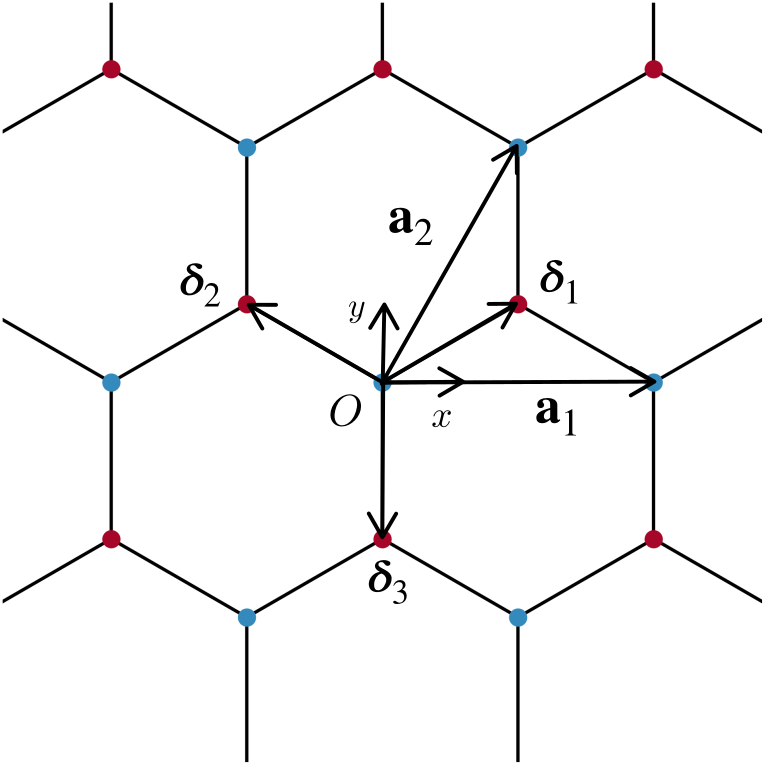
\includegraphics[height=.78\linewidth]{fig/honeycomb_coordinates_deltas.png}
  \caption{Graphene's lattice with atoms labeled $\textcolor{blue}{A}$ (blue) and $\textcolor{red}{B}$ (red), both being identical carbon atoms.}
  \label{fig:graphene-lattice_a}
\end{subfigure} \hfill
\begin{subfigure}{.48\textwidth}
  \centering
  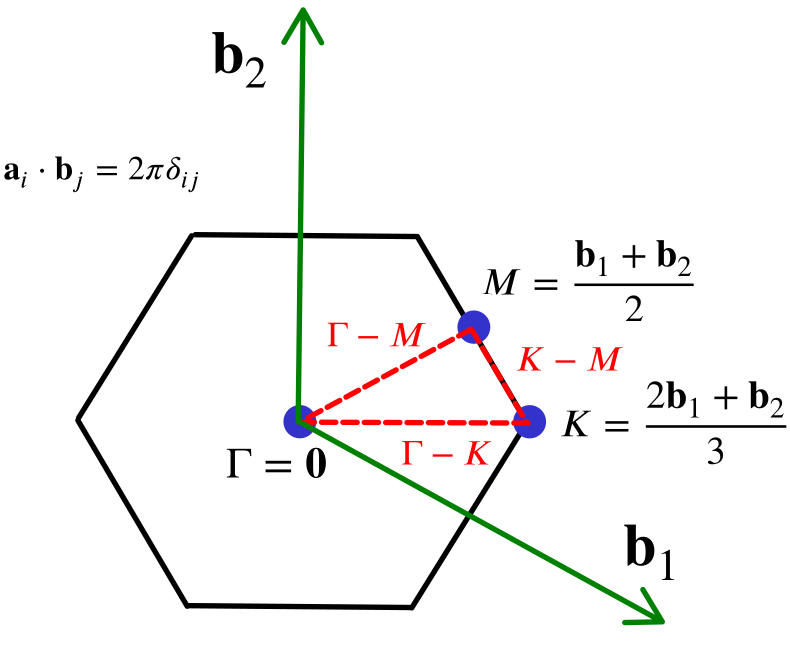
\includegraphics[height=.78\linewidth]{fig/honeycomb_tqc_BZ.png}
  \caption{Graphene Brillouin Zone with high-symmetry momentum points labeled as $\Gamma$, $K$, and $M$.}
  \label{fig:graphene-lattice_b}
\end{subfigure}
%\caption{}
\label{fig:graphene-lattice}
\end{figure}

The lattice vectors are defined as \(\vb{a}_1 = a \qty(1, 0)\) and \(\vb{a}_2 = a \qty(\frac{1}{2}, \frac{\sqrt{3}}{2})\), with $a = d\sqrt{3} = 2.46 \, \AA$. The unit cell area is given by \( A_1 = \abs{\a_1 \times \a_2} = \frac{\sqrt{3}}{2} a^2 \). The momentum lattice vectors \(\b_1\) and \(\b_2\) satisfy the relation \(\a_i \vdot \b_j = 2\pi \delta_{ij}\) and can be derived as follows:
\begin{equation} \label{eq:monolayer-bvecs}
\b_1 = \frac{2\pi}{A_1} \a_2 \times \a_3 = \frac{4\pi}{\sqrt{3} a } \qty(\frac{\sqrt{3}}{2}, -\frac{1}{2}), \quad
\b_2 = \frac{2\pi}{A_1} \a_3 \times \a_1 = \frac{4\pi}{\sqrt{3} a } \qty(0, 1),
\end{equation}
where for calculation purposes, we used \(\a_3 = \vu{z}\).

The two main Dirac points lie at the edge of the Brillouin Zone (BZ), as illustrated in Figure \ref{fig:graphene-lattice_b}, and are defined as:
\begin{equation} \label{eq:monolayer-dirac-points}
K = \frac{2\b_1 + \b_2}{3} = \frac{4\pi}{3a} (1, 0) , \quad K' = -K.
\end{equation}

Ignoring the spin degree of freedom (since spin-orbit coupling is weak in graphene and magnetic fields are not considered), the tight-binding Hamiltonian with only nearest-neighbor hoppings is expressed as:
\begin{equation} \label{eq:monolayer-tight-binding}
H = -t \sum_{\R} c^\d_A(\R) \qty(c_B(\R + \vdelta_1) + c_B(\R+\vdelta_2) + c_B(\R+\vdelta_3)) + \hc,
\end{equation}
where $t = 2.97 \unit{eV}$ according to \textit{ab initio} calculations \cite{handbook2019}, and \(\R = n_1 \a_1 + n_2 \a_2\), with integers \(n_1, n_2\), runs over all the lattice sites of the underlying Bravais triangular lattice. Applying the following Fourier transformation:
\begin{equation} \label{eq:monolayer-fourier}
c_{\alpha}^\d(\r) = \frac{1}{\sqrt{N}} \sum_{\k \in \text{BZ}} e^{-i \k \vdot \r} c_\alpha^\d(\k),
\end{equation}
we obtain the Hamiltonian in momentum space
\begin{equation} \label{eq:monolayer-tight-binding2}
H = \sum_{\k}
\begin{pmatrix}
c_A^\d(\k) & c_B^\d(\k)
\end{pmatrix}
H_\k
\begin{pmatrix}
c_A^\d(\k) \\ c_B^\d(\k)
\end{pmatrix},
\end{equation}
where the matrix \(H_\k\) is
\begin{equation} \label{eq:hamiltonian_k_monolayer}
H_\k =
\begin{pmatrix}
0 & -t f(\k) \\
-t f^{\dagger}(\k) & 0
\end{pmatrix},
\end{equation}
and the function \(f(\k)\) is given by
\begin{equation} \label{eq:monolayer-fk}
f(\k) = e^{i \k \vdot \bm{\delta}_1} + e^{i \k \vdot \bm{\delta}_2} + e^{i \k \vdot \bm{\delta}_3} =
e^{-idk_y} + 2 e^{\frac{idk_y}{2}} \cos(\frac{\sqrt{3}}{2} dk_x),
\end{equation}
where \(\bm{\delta}_1 = \frac{\a_1 + \a_2}{3} = d \qty(\frac{\sqrt{3}}{2}, \frac{1}{2})\), \(\bm{\delta}_2 = \frac{-2 \a_1 + \a_2}{3} = d \qty(-\frac{\sqrt{3}}{2}, \frac{1}{2})\), and \(\bm{\delta}_3 = \frac{\a_1 - 2 \a_2}{3} = d \qty(0, -1)\) are the vectors connecting the three nearest neighbor sites.

The eigenenergies of the Hamiltonian matrix \(H_\k\) are \(E_\pm(\k) = \pm t \abs{f(\k)}\). The Dirac points \(K\) and \(K' = -K\) correspond to the zeros of \(f(\k)\), i.e., \(f(\pm K) = 0\). In the vicinity of these points, the dispersion relation is approximately linear, as illustrated in Figure \ref{fig:monolayer_dispersion}.
\begin{equation} \label{eq:linear_Ek_monolayer}
E(\K + \q) = v_0 \abs{\q} + O\left(\frac{\abs{\q}}{\abs{K}}\right)^2,
\end{equation}
where \( v_0 = \frac{3td}{2} \) is the Fermi velocity, adopting the convention \(\hbar = 1\). The \(p_z\) electrons in graphene exhibit a dispersion relation analogous to that of relativistic Dirac particles, though their velocity, \(v_0 \approx 10^6 \, \text{m/s}\), is approximately 300 times smaller than the speed of light, \(c = 3 \times 10^8 \, \text{m/s}\).

\begin{figure}[H]
\centering
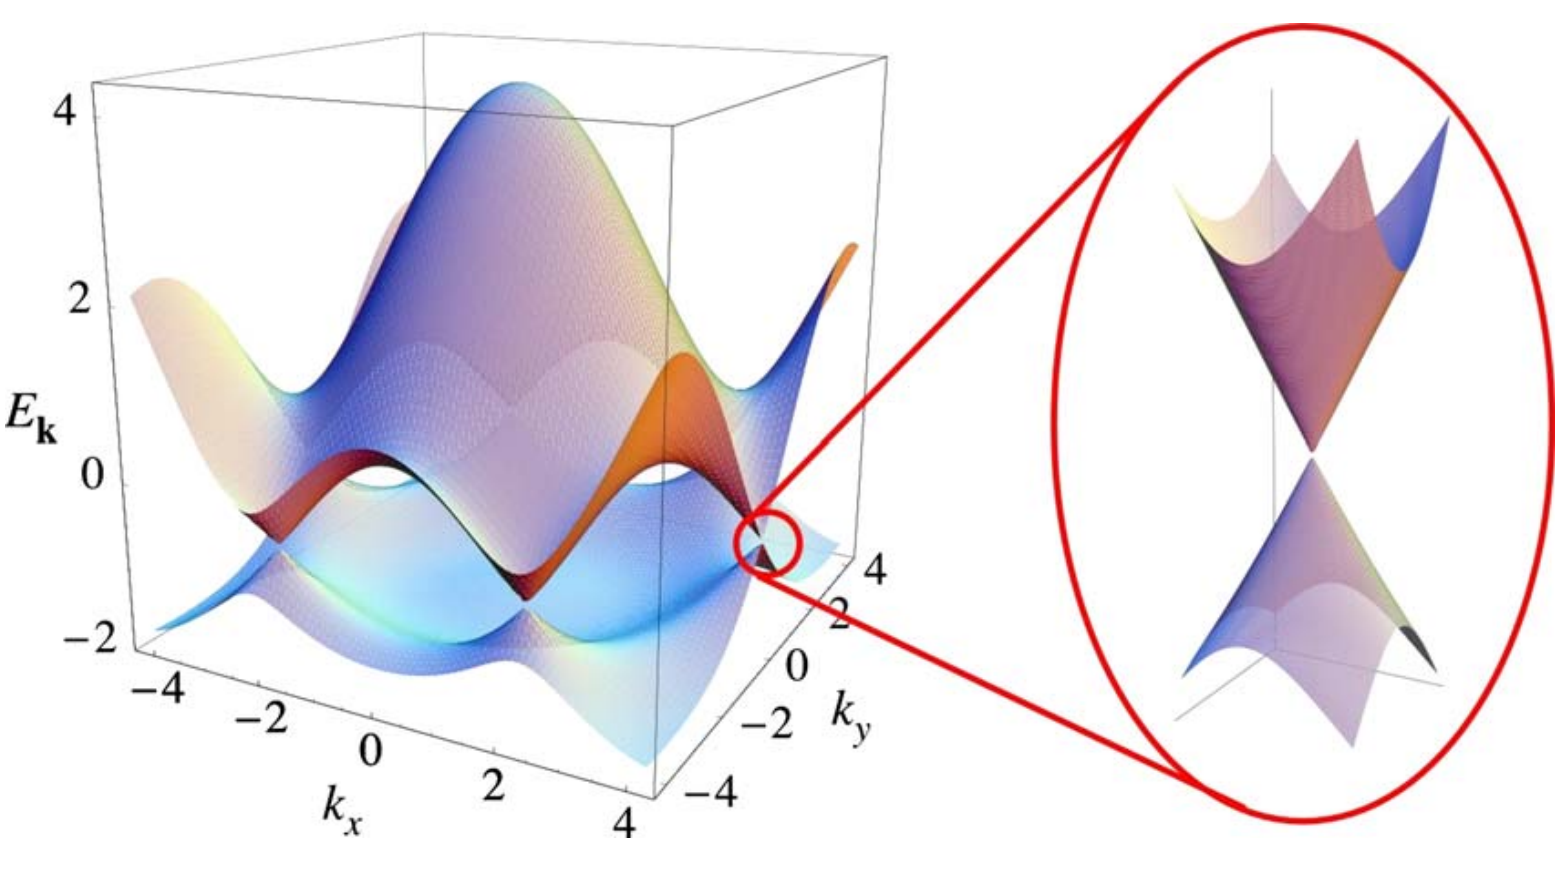
\includegraphics[width=0.8\linewidth]{fig/monolayer_dispersion.png}
\caption{Electronic band structure of graphene (energy in eV). Adapted from \cite{geim2009}.}
\label{fig:monolayer_dispersion}
\end{figure}

%%%%%%%%%%%%%%%%%%%%%%%%%%%%%%%%%%%%%%%%%%%%%%%%%%%%%%%%%%%%%%%%%%%%%%%%%%%%%%%%%%%%%%%%%%%%%%%%%%
\section{Twisted bilayer graphene} \label{sec:experimental_tbg}
%%%%%%%%%%%%%%%%%%%%%%%%%%%%%%%%%%%%%%%%%%%%%%%%%%%%%%%%%%%%%%%%%%%%%%%%%%%%%%%%%%%%%%%%%%%%%%%%%%

Twisted bilayer graphene (TBG), formed by stacking two graphene layers with a small twist angle, has become a highly researched material due to its rich and highly tunable electronic properties. The twist between the layers gives rise to a moiré pattern, as illustrated in Figure \ref{fig:moire_pattern}, which introduces a complex modulation of the interlayer interactions. This modulation significantly alters the band structure compared to that of monolayer graphene, as previously shown in Figure \ref{fig:monolayer_dispersion}.
%\begin{figure}[H]
%\centering
%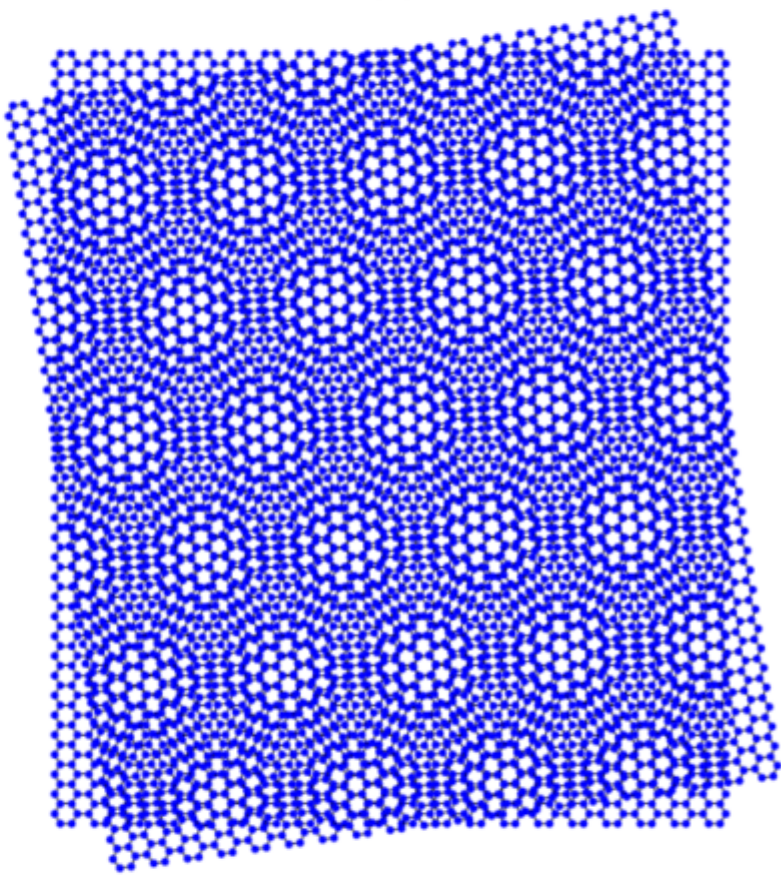
\includegraphics[width=0.4\linewidth]{fig/moire_pattern.png}
%\caption{Moiré pattern.}
%\label{fig:moire_pattern}
%\end{figure}

\begin{figure}[H]
\centering
\begin{subfigure}{.37\textwidth}
  \centering
  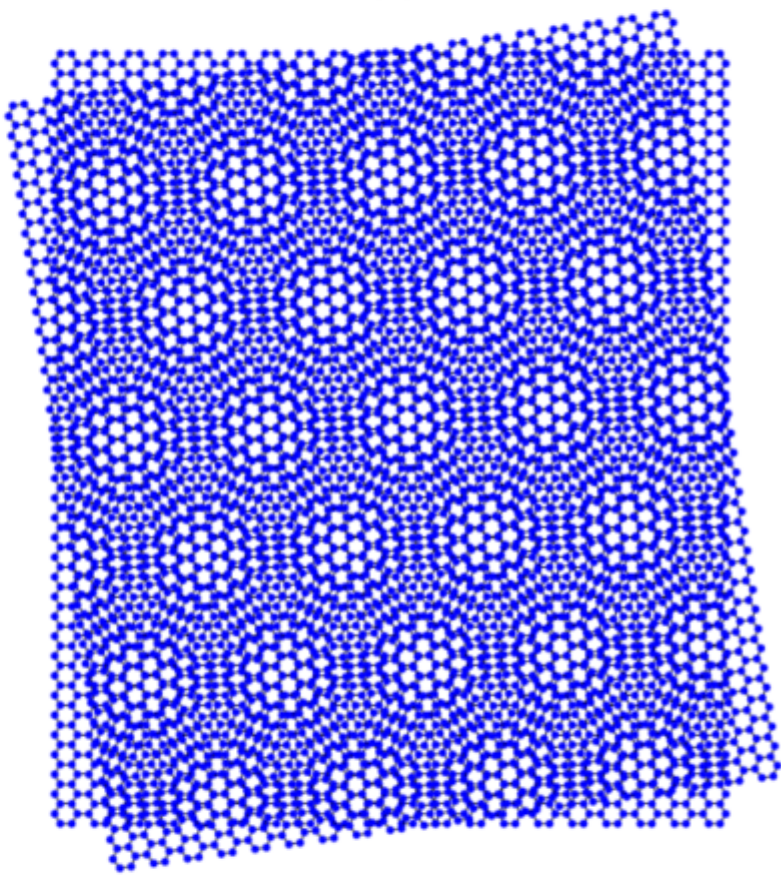
\includegraphics[height=12em]{fig/moire_pattern.png}
  \caption{Moiré pattern formed by two twisted graphene layers. Adapted from \cite{moire_pattern_figure2021}.}
  \label{fig:moire_pattern}
\end{subfigure} \hfill
\begin{subfigure}{.60\textwidth}
  \centering
  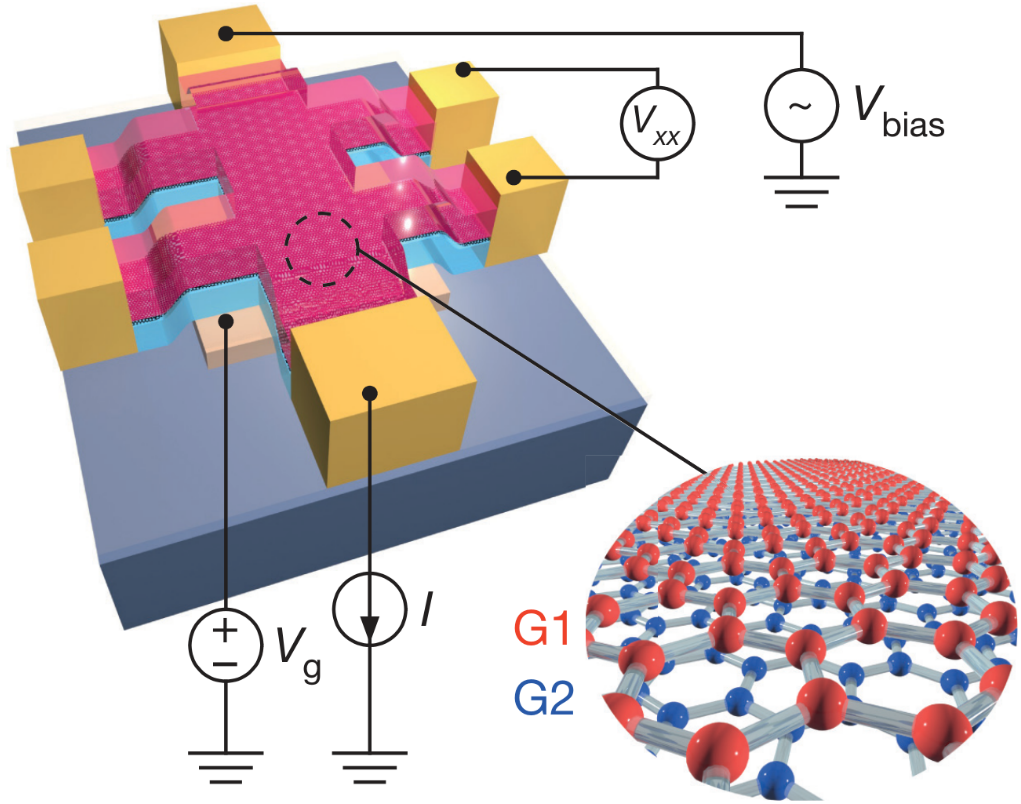
\includegraphics[height=11em]{fig/tbg_device2.png}
  \caption{Schematic of a TBG device with a four-probe setup. Hexagonal boron nitride (hBN) layers encapsulates the TBG, and a metal gate below the bottom hBN controls electron density. Adapted from \cite{cao2018}.}
  \label{fig:tbg_device2}
\end{subfigure}
\caption{Illustration of the TBG system, depicting the moiré pattern and the experimental setup.}
\label{fig:tbg_moire_device}
\end{figure}

%\begin{figure}[H]
%\centering
%\begin{subfigure}{.37\textwidth}
%  \centering
%  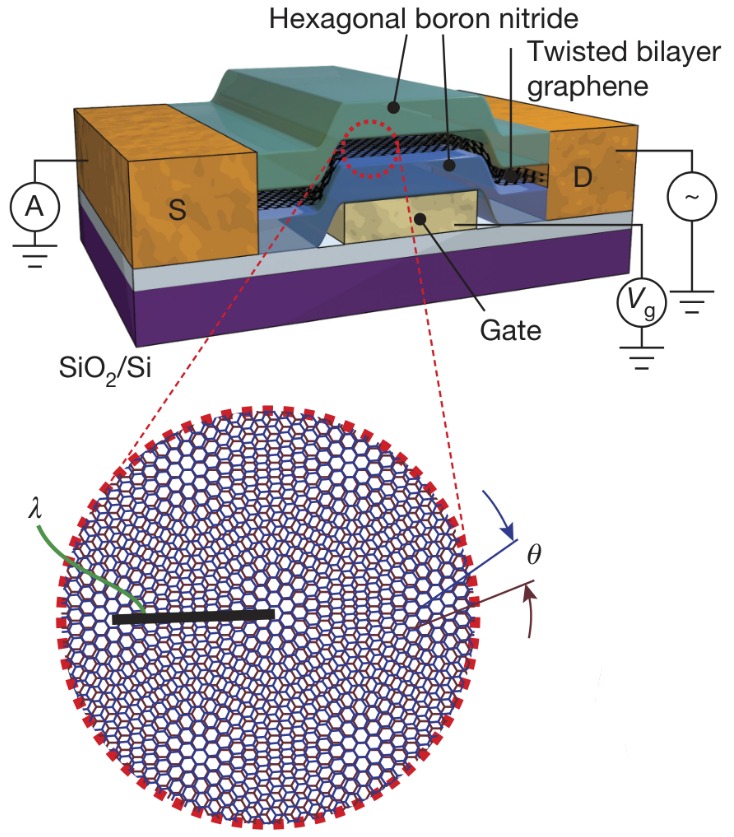
\includegraphics[height=10em]{fig/tbg_device.png}
%  \caption{Schematic of the TBG devices. The TBG is encapsulated in hBN flakes and fabricated on SiO$_2$/Si substrates.}
%  \label{fig:tbg_device}
%\end{subfigure} \hfill
%\begin{subfigure}{.60\textwidth}
%  \centering
%  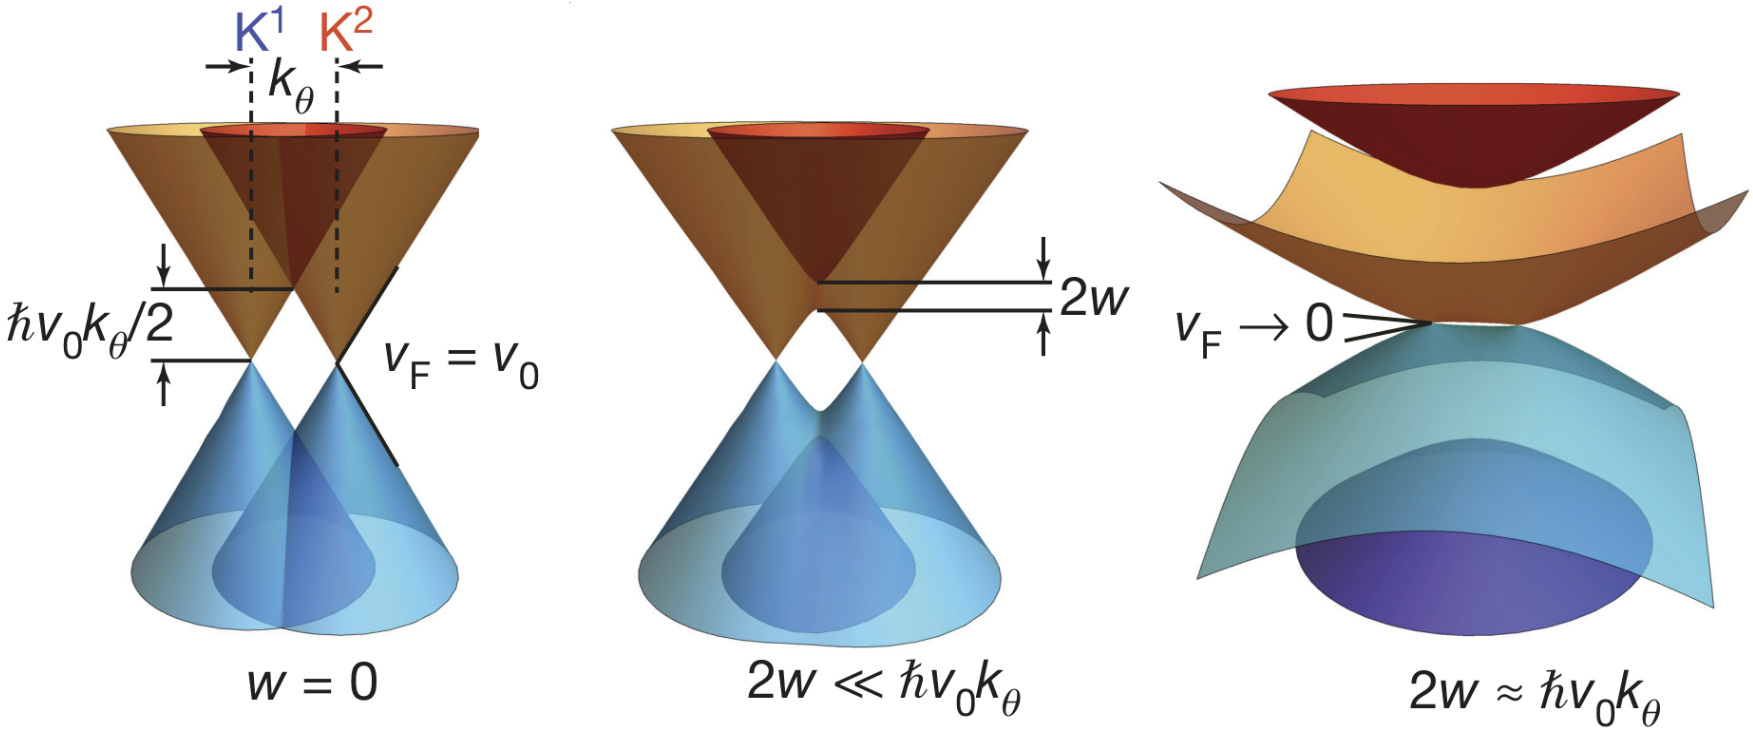
\includegraphics[height=10em]{fig/tbg_dirac_cones.png}
%  \caption{Illustration of the effect of interlayer hybridization: \( w = 0 \), \( 2w \ll \hbar v_0 k_\theta \), and \( 2w \approx \hbar v_0 k_\theta \), where \( v_0 = 10^6 \, \text{m/s} \) is the Fermi velocity of graphene.}
%  \label{fig:tbg_dirac_cones}
%\end{subfigure}
%\caption{Both figures were taken from \cite{cao2018_correlated}.}
%\label{fig:tbg_figures_taken_from_correlated_insul}
%\end{figure}

At specific twist angles, known as \textit{magic angles}, these interactions give rise to nearly flat electronic bands near the charge neutrality point (CNP), separated from other bands by gaps on the order of tens of meV. This band flattening is a result of the interplay between intra- and interlayer hybridization energies, as shown in Figure \ref{fig:tbg_dirac_cones}. It occurs when the energy \(2w\), associated with interlayer coupling, becomes comparable to the energy difference \(\hbar v_0 k_\theta\) between the Dirac cones at the \(K^{(1)}\) and \(K^{(2)}\) points of the two layers.

\begin{figure}[H]
\centering
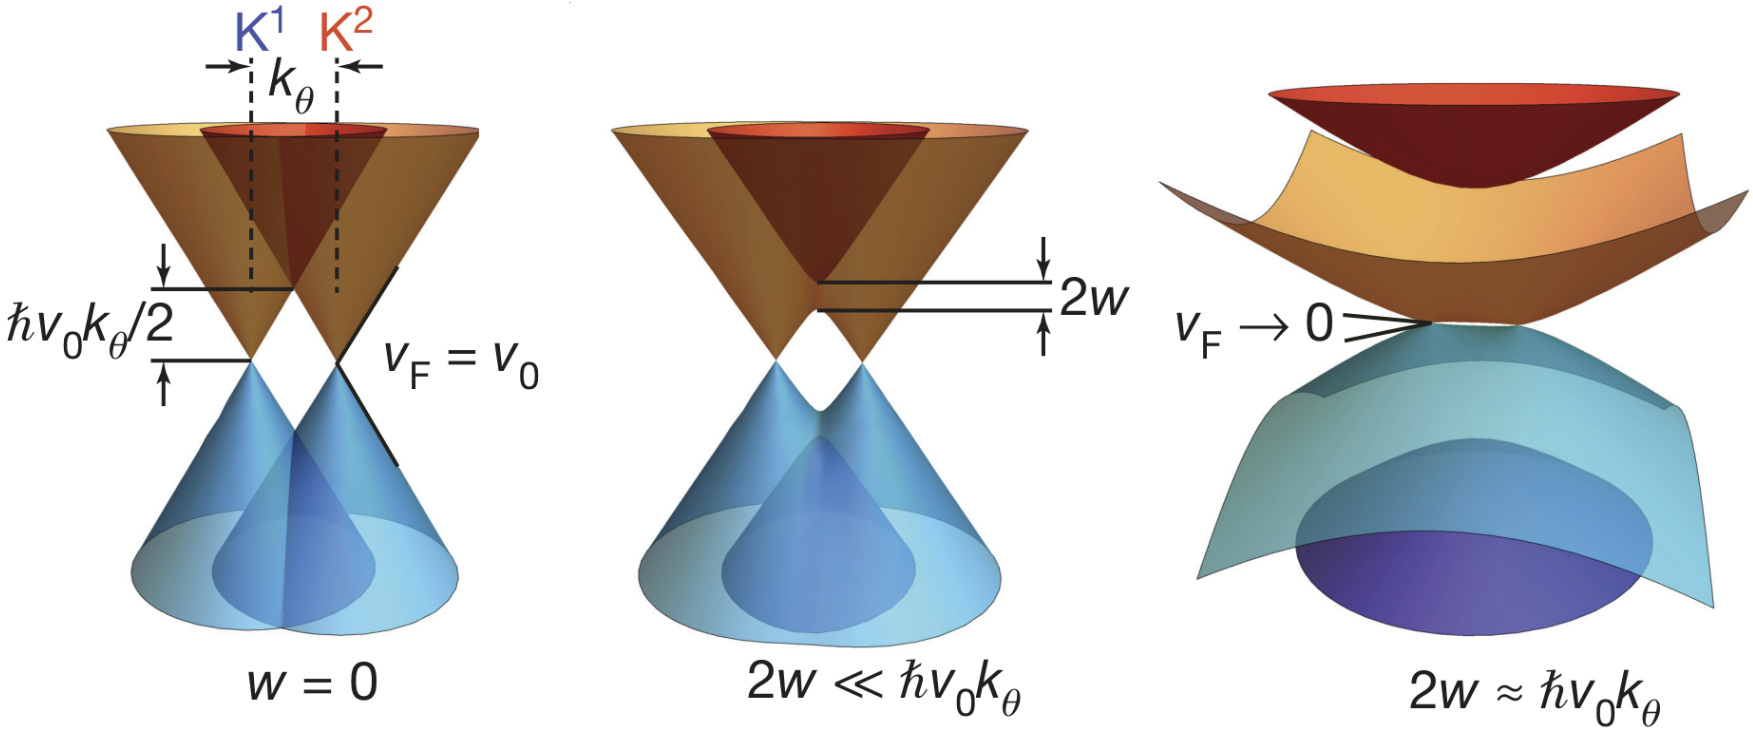
\includegraphics[width=0.60\linewidth]{fig/tbg_dirac_cones}
\caption{Illustration of interlayer hybridization in three scenarios: (1) \( w = 0 \), no interlayer coupling; (2) \( 2w \ll \hbar v_0 k_\theta \), weak interlayer coupling; and (3) \( 2w \approx \hbar v_0 k_\theta \), strong interlayer coupling. Here, \( v_0 \approx 10^6 \, \text{m/s} \) is the Fermi velocity of graphene and $k_\theta = 2 \abs{K} \sin(\theta/2)$. Adapted from \cite{cao2018_correlated}.}
\label{fig:tbg_dirac_cones}
\end{figure}

At twist angles near the magic angles, a variety of extraordinary phenomena emerge. Bistritzer and MacDonald \cite{macdonald2011} predicted that the hybridization of Dirac cones at the \(K\) and \(K'\) points leads to the opening of energy gaps at their intersections and a significant renormalization of the Fermi velocity. At the magic angles, the Fermi velocity vanishes, giving rise to isolated, narrow bands around the charge neutrality point (CNP). These near flat bands are a hallmark of twisted bilayer graphene (TBG) and have been experimentally confirmed, particularly at the first magic angle (\(\theta \approx 1.1^\circ\)), where four extremely narrow bands appear at the CNP, as illustrated in Figures \ref{fig:tbg_bandstructure_a} and \ref{fig:tbg_bandstructure_b}.

\begin{figure}[H]
\centering
\begin{subfigure}{.48\textwidth}
  \centering
  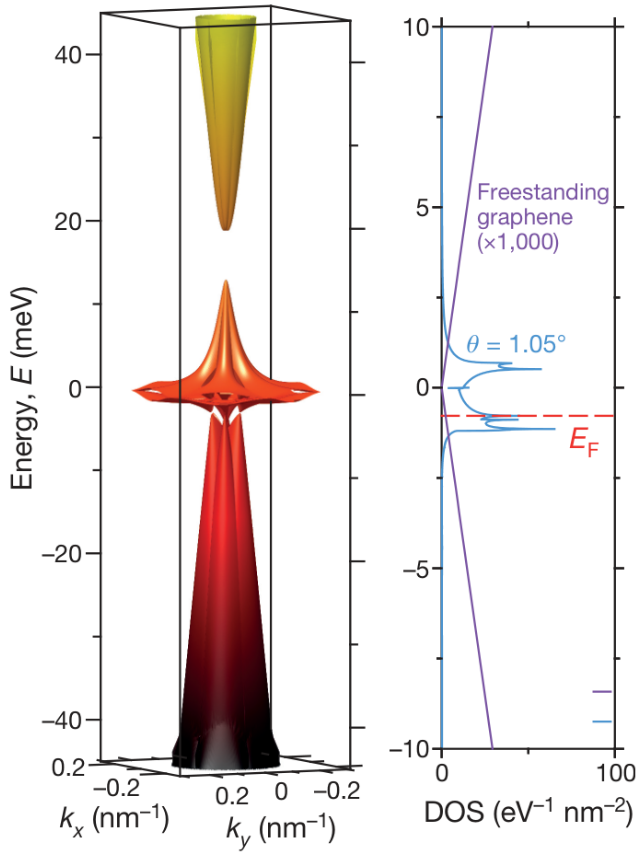
\includegraphics[height=20em]{fig/tbg_bandstructure.png}
  \caption{Band structure of TBG in \((k_x, k_y)\) momentum space within the mBZ at \(\theta = 1.05^\circ\), along with its corresponding density of states. Adapted from \cite{cao2018}.}
  \label{fig:tbg_bandstructure_a}
\end{subfigure} \hfill
\begin{subfigure}{.48\textwidth}
  \centering
  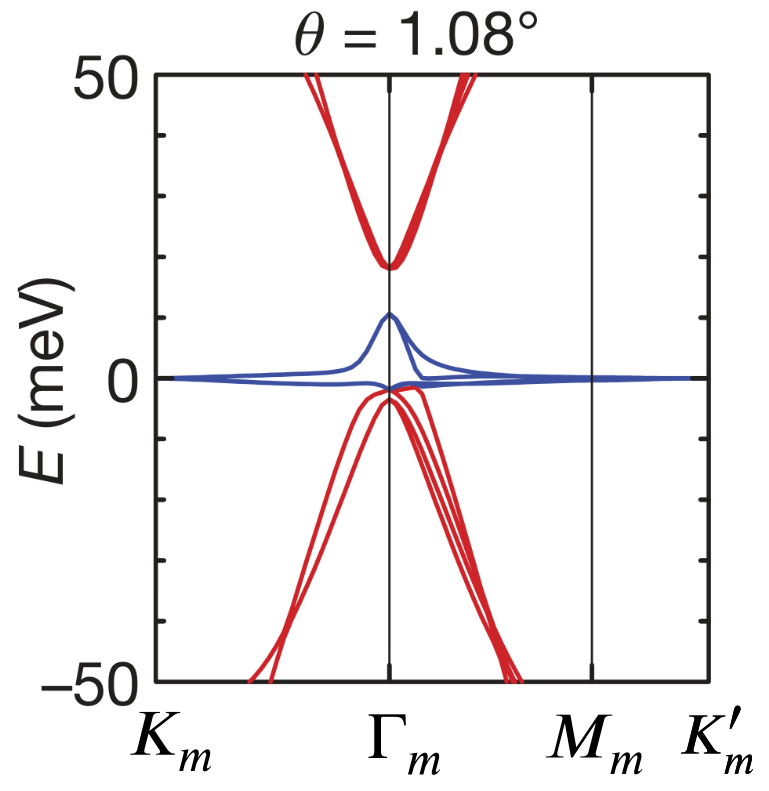
\includegraphics[height=21em]{fig/tbg_4_narrowbands.png}
  \caption{Four narrow bands at angle \(\theta = 1.08^\circ\), with the bandstructure plotted along the high-symmetry lines \(\Gamma_m - K_m - M_m - K_m'\) in the mBZ. Adapted from \cite{cao2018_correlated}.}
  \label{fig:tbg_bandstructure_b}
\end{subfigure}
\caption{Band structure of TBG in the mini Brillouin Zone (mBZ), showing the appearance of flat bands near the charge neutrality point (CNP) near the magic angle $\theta \approx 1.1^\circ$.}
\label{fig:tbg_figures_taken_from_correlated_insul}
\end{figure}


Jarillo-Herrero et al. \cite{cao2018, cao2018_correlated} discovered that doping the flat bands in TBG leads to the emergence of both insulating and superconducting phases, marking a new frontier in two-dimensional materials research. The insulating states, observed at half-fillings of the flat bands in Figure \ref{fig:tbg_conductance_filling_insulating}, are Mott insulators, driven by electron-electron interactions rather than band theory alone. These states are characterized by a sharp drop in conductance, indicating a transition from metallic to insulating behavior, with conductance exponentially suppressed below a critical temperature of approximately \(T_c = 4 \, \text{K}\), as shown in Figure \ref{fig:tbg_conductance_temperature_insulating}.

\begin{figure}[H]
\centering
\begin{subfigure}{.56\textwidth}
  \centering
  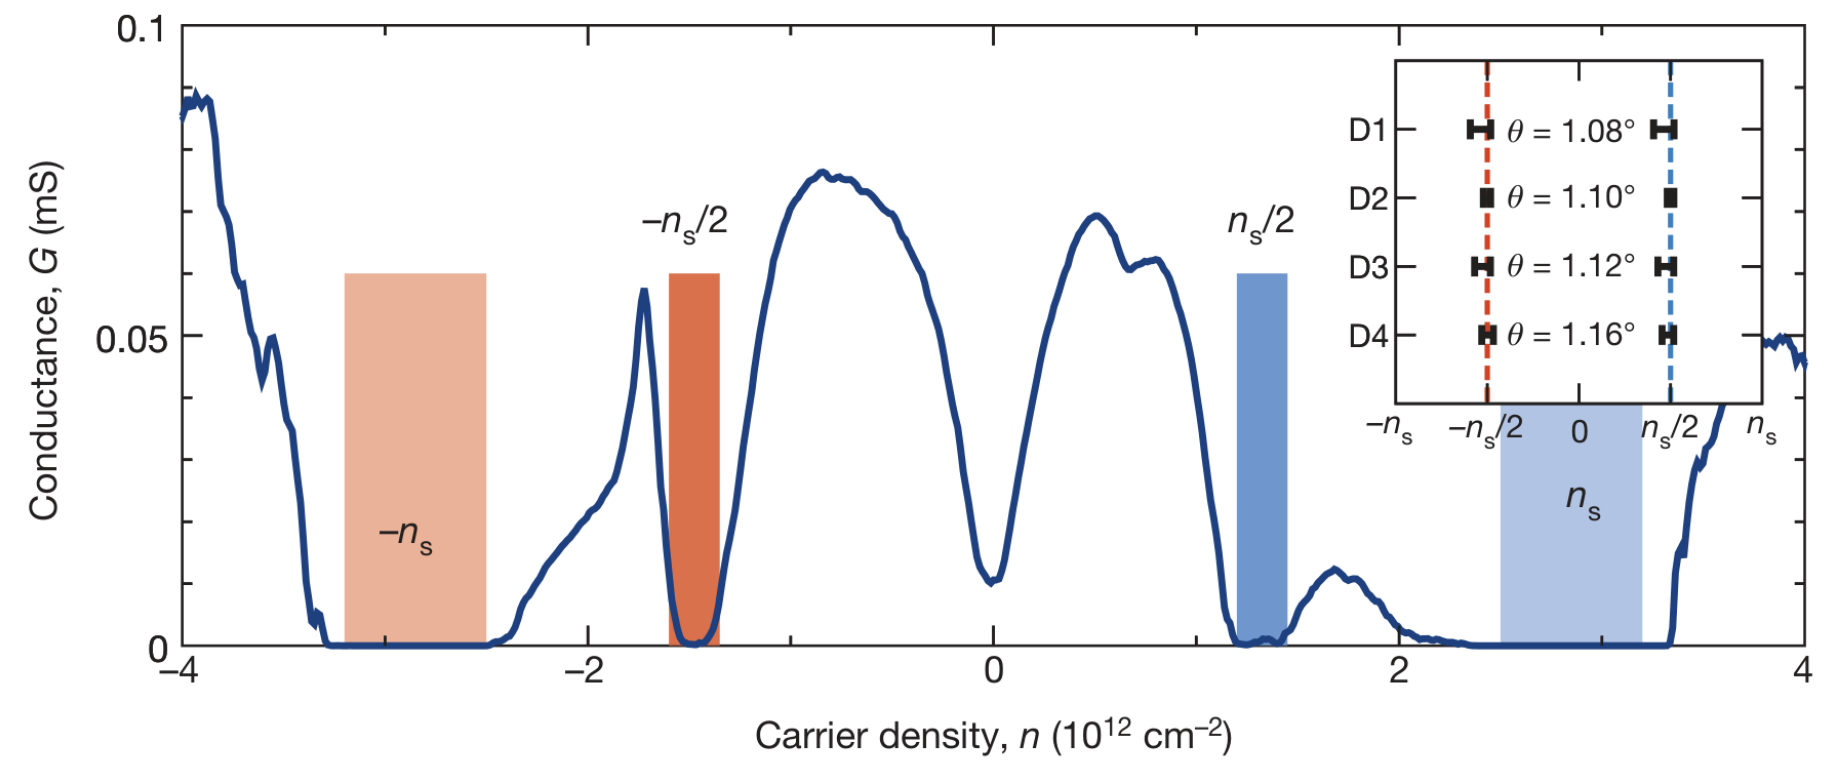
\includegraphics[height=9.5em]{fig/tbg_conductance_filling_insulating.png}
  \caption{Half-filling insulating states in MATBG. Conductance \(G\) of a TBG device with \(\theta = 1.08^\circ\) at \(T = 0.3 \, \text{K}\). Lighter-shaded regions indicate superlattice gaps at carrier density \(n = \pm n_s = \pm 2.7 \times 10^{12} \, \text{cm}^{-2}\), and darker-shaded regions show half-filling insulating states at \(n = \pm n_s/2\). Inset displays half-filling state positions across four devices.}
  \label{fig:tbg_conductance_filling_insulating}
\end{subfigure} \hfill
\begin{subfigure}{.40\textwidth}
  \centering
  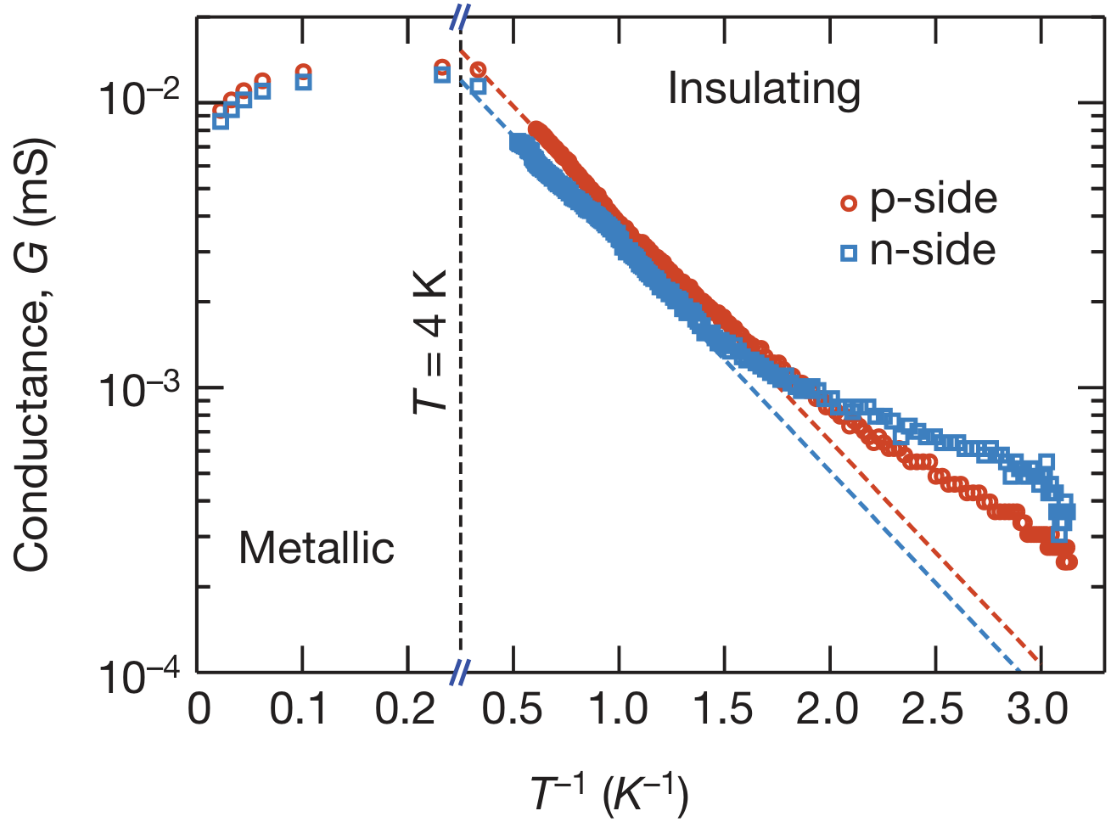
\includegraphics[height=9.5em]{fig/tbg_conductance_temperature_insulating.png}
  \caption{Minimum conductance in half-filling states at $\theta = 1.08^\circ$ for the \(p\)-side (red) and \(n\)-side (blue) of the device. The dashed lines represent exponential fits of the form \(\exp[-\Delta/(2kT)]\), with \(\Delta \approx 0.31 \, \text{meV}\) being the thermal activation gap.}
  \label{fig:tbg_conductance_temperature_insulating}
\end{subfigure}
\caption{Evidence of half-filling insulating states at the magic angle \(\theta = 1.08^\circ\). Adapted from \cite{cao2018_correlated}.}
\label{fig:tbg_insulating}
\end{figure}

%The fabrication of TBG devices involves a "tear and stack" technique, which enables precise control of the twist angle with accuracies on the order of \(0.1^\circ\)-\(0.2^\circ\). These devices are typically encapsulated in hexagonal boron nitride (hBN) to protect them from environmental effects and fabricated on SiO\(_2\)/Si substrates. A bottom Pd/Au gate is employed to control the charge carrier density, allowing for precise doping of the material. These advancements in fabrication techniques have been critical in probing the unique physics of TBG, including its insulating and superconducting behaviors.

%In terms of theoretical modeling, various approaches—including tight-binding and continuum models—have been employed to calculate the electronic band structure of tBLG. For small twist angles (typically between 1$^\circ$ and 2$^\circ$), these models predict a significant reduction in the Fermi velocity, which tends to zero at the magic angle. The energy dispersion around the K and K' points is not linear, and the hybridization of Dirac cones results in a pair of Van Hove singularities in the density of states. As the twist angle decreases, the interlayer hopping energy, denoted as \(t_\theta\), becomes comparable to the energy difference between the cones, pushing the intersection of the cones to zero energy.

%A particularly interesting feature of tBLG is the formation of a Mott-like insulator phase at half-filling of the moiré unit cell. The correlated insulating states observed near half-filling are consistent with theoretical predictions based on the interplay between the Coulomb interaction and the suppression of kinetic energy due to the flat bands near magic angles. This Mott-like insulating behavior can be confirmed by temperature-dependent conductance measurements, which show a transition from a metallic phase at higher temperatures to an insulating phase at low temperatures.

Also upon slight doping away from these insulating states, the system exhibits superconducting behavior, with a critical temperature in the range of a few Kelvins. This superconductivity, which emerges at doping levels near half-filling, has similarities to high-temperature superconductivity observed in cuprates, and has stimulated extensive theoretical and experimental investigations. The phase diagram of tBLG reveals superconducting domes surrounding the insulating phase, with the system transitioning to a normal metallic state at higher temperatures or under the application of a magnetic field.

Scanning tunneling microscopy (STM) has provided valuable insights into the local density of states (LDOS) and the evolution of the flat bands as the system is doped away from the charge neutrality point. These experiments show that the bandwidth of the flat bands increases as the chemical potential is tuned closer to the CNP, with a maximum bandwidth observed at charge neutrality. Furthermore, STM studies have revealed breaking of the three-fold rotational symmetry in the system when doped around quarter filling, indicating the potential emergence of new symmetries and topological phenomena in tBLG.

The application of a magnetic field to tBLG devices has also been shown to affect the insulating and superconducting phases. At high magnetic fields (\(B \approx 4T\)), the insulating states are suppressed, and the system enters a metallic phase. The Zeeman energy required to suppress the insulating states is approximately 0.5 meV, which is consistent with the thermal activation gap observed in low-temperature measurements. The combination of strong electron-electron interactions, superconductivity, and topological phenomena observed in tBLG makes it a promising material for exploring new quantum phases and understanding the complex behavior of correlated electron systems in two dimensions.

In conclusion, the study of twisted bilayer graphene presents a fascinating and multifaceted exploration of two-dimensional materials, with applications spanning superconductivity, Mott insulators, and topological phenomena. The ability to control the twist angle with high precision, along with the discovery of superconductivity in the absence of traditional pairing mechanisms, makes tBLG an exciting material for future research in condensed matter physics.

In terms of theoretical modeling, various approaches—including tight-binding and continuum models—have been employed...

\n
\textbf{OUTRA VERSÃO DO CHATGPT}
\n

Twisted bilayer graphene (tBLG) exhibits some of the most striking and profound moiré phenomena, especially when two graphene layers are slightly twisted relative to each other. This twist leads to an interlayer coupling whose strength is modulated by the local registry between the two layers, varying gradually according to the long-wavelength moiré pattern. The resulting low-energy band structure of tBLG reveals two sets of monolayer graphene Dirac cones rotated by the twist angle \(\theta\) (Fig. 1.1(b)), with the interlayer hybridization mixing the Dirac cones at either the \(K\) or \(K'\) valleys. Bistritzer and MacDonald (Ref. [11]) predicted that this hybridization induces energy gaps near the intersection of the Dirac cones and a significant renormalization of the Fermi velocity \(v_F\). At specific twist angles, termed "magic angles," the Fermi velocity vanishes, and the associated moiré bands become extremely flat, with bandwidths reduced to tens of meV. This flattening arises due to the competition between intra- and interlayer hybridization energy strengths (Fig. 1.1(b-d)).

At the first magic angle (\(\theta \approx 1.1^\circ\)), the band structure, as shown in Fig. 1.1(f), exhibits four narrow, isolated bands centered around the charge neutrality point (CNP). Cao et al. (Ref. [8], [9]) discovered that doping these bands opened a new frontier in the study of 2D materials, moiré superlattices, insulating and superconducting states, emergent symmetries, and topological phenomena. The devices were fabricated using the "tear and stack" method, which ensures precise control over the twist angle (accuracy of \(0.1^\circ - 0.2^\circ\)), and encapsulated in hexagonal boron nitride (hBN) flakes on SiO\(_2\)/Si substrates (Fig. 1.1(a)). A bottom Pd/Au gate was used to control the charge carrier density.

Fig. 1.2(a) presents the conductance as a function of charge carrier density, showing metallic behavior as the chemical potential is shifted away from the CNP. However, as the system reaches quarter-integer fillings of \(\pm 2\) electrons per unit cell, the conductance drops sharply, indicating a transition to an insulating state. Temperature-dependent conductance measurements in Fig. 1.2(b) show exponential suppression of conductance below approximately 4 K, consistent with an activation gap \(\Delta \approx 0.3 \, \text{meV}\). Further, applying a perpendicular magnetic field (Fig. 1.2(c)) converts these insulating states into metallic ones, with the Zeeman energy required to suppress the insulating states matching the thermal activation energy. These insulating states are thought to be Mott insulators, driven by electron-electron interactions, rather than single-particle effects predicted by band structure calculations.

The insulator-metal transition and superconductivity in tBLG have been subjects of intense study. Upon slight doping away from the insulating phase, conductance sharply increases, with resistance dropping to zero—indicative of superconductivity. The superconducting critical temperature is a few Kelvins, and the state can be suppressed by a magnetic field of 0.4 Tesla. The phase diagram around quarter filling (Fig. 1.2(d)) reveals two superconducting domes surrounding the insulating state, similar to the phase diagram observed in cuprate superconductors, which has spurred both experimental and theoretical efforts to understand the underlying mechanisms.

Recent improvements in sample quality and experimental setups have expanded the phase diagram, with insulating states observed at other integer fillings of the flat bands, including charge neutrality (Refs. [14]-[20]). At a filling of \(\nu = \pm 3\), an intriguing magnetic phase emerges, where longitudinal resistance approaches the quantized Hall value \(\frac{\hbar}{e^2}\) and exhibits hysteresis, signaling the Quantum Anomalous Hall effect. This behavior suggests spontaneous time-reversal symmetry breaking and points to a topological origin.

Scanning tunneling microscopy (STM) studies have provided insights into the local and total density of states near the magic angle, with the density of states exhibiting a pronounced peak at the AA stacking regions of the moiré pattern (Refs. [16], [17], [18]). Additionally, the separation between van Hove singularities increases as the chemical potential moves within the flat bands, peaking at the CNP. Furthermore, a three-fold rotational symmetry breaking has been observed when doping near the quarter-filling insulating phase (Refs. [16], [20], [17]).

Another fascinating feature of tBLG is the large linear-in-temperature resistivity, which persists over a broad range of twist angles and up to several tens of Kelvins (Refs. [23], [24]). This behavior is attributed to electron-phonon scattering (Refs. [23], [25]) or quantum fluctuations (Ref. [24]).

Superconductivity has been observed across a broader range of doping densities, even when insulating states are suppressed, either by the proximity of a metallic layer (Ref. [27]) or by slight deviation from the magic angle (Ref. [26]). The fact that superconductivity arises in the absence of correlated insulating states suggests that it originates independently and might be explained by the standard BCS electron–phonon coupling mechanism (Refs. [28], [29], [30]).

Calculations of the tBLG band structure have been performed using methods such as tight-binding and continuum approximations, as well as more advanced ab initio approaches (Refs. [10], [16], [17], [18], [24], [26], [27]). These calculations consistently predict that for small twist angles, especially near the magic angles, four nearly flat bands emerge near the charge neutrality point, with a bandwidth on the order of 10–20 meV (Fig. 1.15(a)).

For twist angles between \(2^\circ\) and \(15^\circ\), the mini-band dispersion around the K and K' points remains linear, but the Fermi velocity decreases with decreasing twist angle (Refs. [18], [19]). This behavior is explained by the hybridization of the Dirac cones at the K points, leading to a saddle point in the energy dispersion and the appearance of van Hove singularities in the density of states (Fig. 1.16). As the twist angle decreases, the Fermi velocity approaches zero at the magic angle (\(\theta \approx 1.1^\circ\)) and oscillates for smaller angles (Refs. [17], [18], [20]).

The first magic angle can be estimated by balancing the interlayer hopping energy \(t_\theta\) and the energy scale of the Dirac cones \(v_F k_\theta\), where \(v_F\) is the Fermi velocity, and \(k_\theta\) is the wavevector at the K point (Eq. 1.48). This yields an estimated value of \(\theta \approx 1.1^\circ\), which matches the experimental observation (Ref. [20]). Near this magic angle, the local density of states at the AA stacking regions is highly peaked, and the resulting quenching of the quantum kinetic energy gives rise to a correlated insulating phase at half-filling of the moiré unit cell, resembling a Mott insulator.

In conclusion, the interplay between twist angle, electron-electron interactions, and the resulting moiré patterns in tBLG leads to a rich and tunable phase diagram, with insulating, metallic, and superconducting phases emerging in a manner reminiscent of strongly correlated systems such as cuprate superconductors. This presents exciting opportunities for exploring novel quantum phases in two-dimensional materials.

<++> <++> <++> <++> <++> <++> <++> <++> <++> <++> <++> <++> <++> <++> <++>

%%%%%%%%%%%%%%%%%%%%%%%%%%%%%%%%%%%%%%%%%%%%%%%%%%%%%%%%%%%%%%%%%%%%%%%%%%%%%%%%%%%%%%%%%%%%%%%%%%
\section{Structure of the thesis} \label{sec:outline_thesis}
%%%%%%%%%%%%%%%%%%%%%%%%%%%%%%%%%%%%%%%%%%%%%%%%%%%%%%%%%%%%%%%%%%%%%%%%%%%%%%%%%%%%%%%%%%%%%%%%%%


%%%%%%%%%%%%%%%%%%%%%%%%%%%%%%%%%%%%%%%%%%%%%%%%%%%%%%%%%%%%%%%%%%%%%%%%%%%%%%%%%%%%%%%%%%%%%%%%%%
%%%%%%%%%%%%%%%%%%%%%%%%%%%%%%%%%%%%%%%%%%%%%%%%%%%%%%%%%%%%%%%%%%%%%%%%%%%%%%%%%%%%%%%%%%%%%%%%%%


%%%%%%%%%%%%%%%%%%%%%%%%%%%%%%%% COMMENT THIS TO COMPILE main.tex %%%%%%%%%%%%%%%%%%%%%%%%%%%%%%%%
%%-----
%% Referências bibliográficas
%%-----
\addcontentsline{toc}{chapter}{\bibname}
%\bibliographystyle{abntex2-num}
\bibliography{citations}
\bibliographystyle{ieeetr}
\end{document}
%%%%%%%%%%%%%%%%%%%%%%%%%%%%%%%% COMMENT THIS TO COMPILE main.tex %%%%%%%%%%%%%%%%%%%%%%%%%%%%%%%%
